\documentclass[ngerman,12pt]{scrreprt}

\usepackage{babel}
\usepackage{blindtext}
\usepackage{microtype}
\usepackage{graphicx}
\usepackage{amsmath}
\usepackage{esvect} % \vv{} Befehl

\author{Uwe Ziegenhagen}
\title{Meine Dissertation}

\usepackage{hyperref}
\hypersetup{
    bookmarks=true,                     % show bookmarks bar
    unicode=false,                      % non - Latin characters in Acrobat’s bookmarks
    pdftoolbar=true,                        % show Acrobat’s toolbar
    pdfmenubar=true,                        % show Acrobat’s menu
    pdffitwindow=false,                 % window fit to page when opened
    pdfstartview={FitH},                    % fits the width of the page to the window
    pdftitle={My title},                        % title
    pdfauthor={Author},                 % author
    pdfsubject={Subject},                   % subject of the document
    pdfcreator={Creator},                   % creator of the document
    pdfproducer={Producer},             % producer of the document
    pdfkeywords={keyword1, key2, key3},   % list of keywords
    pdfnewwindow=true,                  % links in new window
    colorlinks=true,                        % false: boxed links; true: colored links
    linkcolor=blue,                          % color of internal links
    filecolor=blue,                     % color of file links
    citecolor=blue,                     % color of file links
    urlcolor=blue                        % color of external links
}

\begin{document}

\maketitle

\tableofcontents

\chapter{Einführung}

\blindtext[2] 

Siehe Abbildung \ref{fig:mieze}, Gleichung \ref{eq:sinnlos}

\begin{figure}
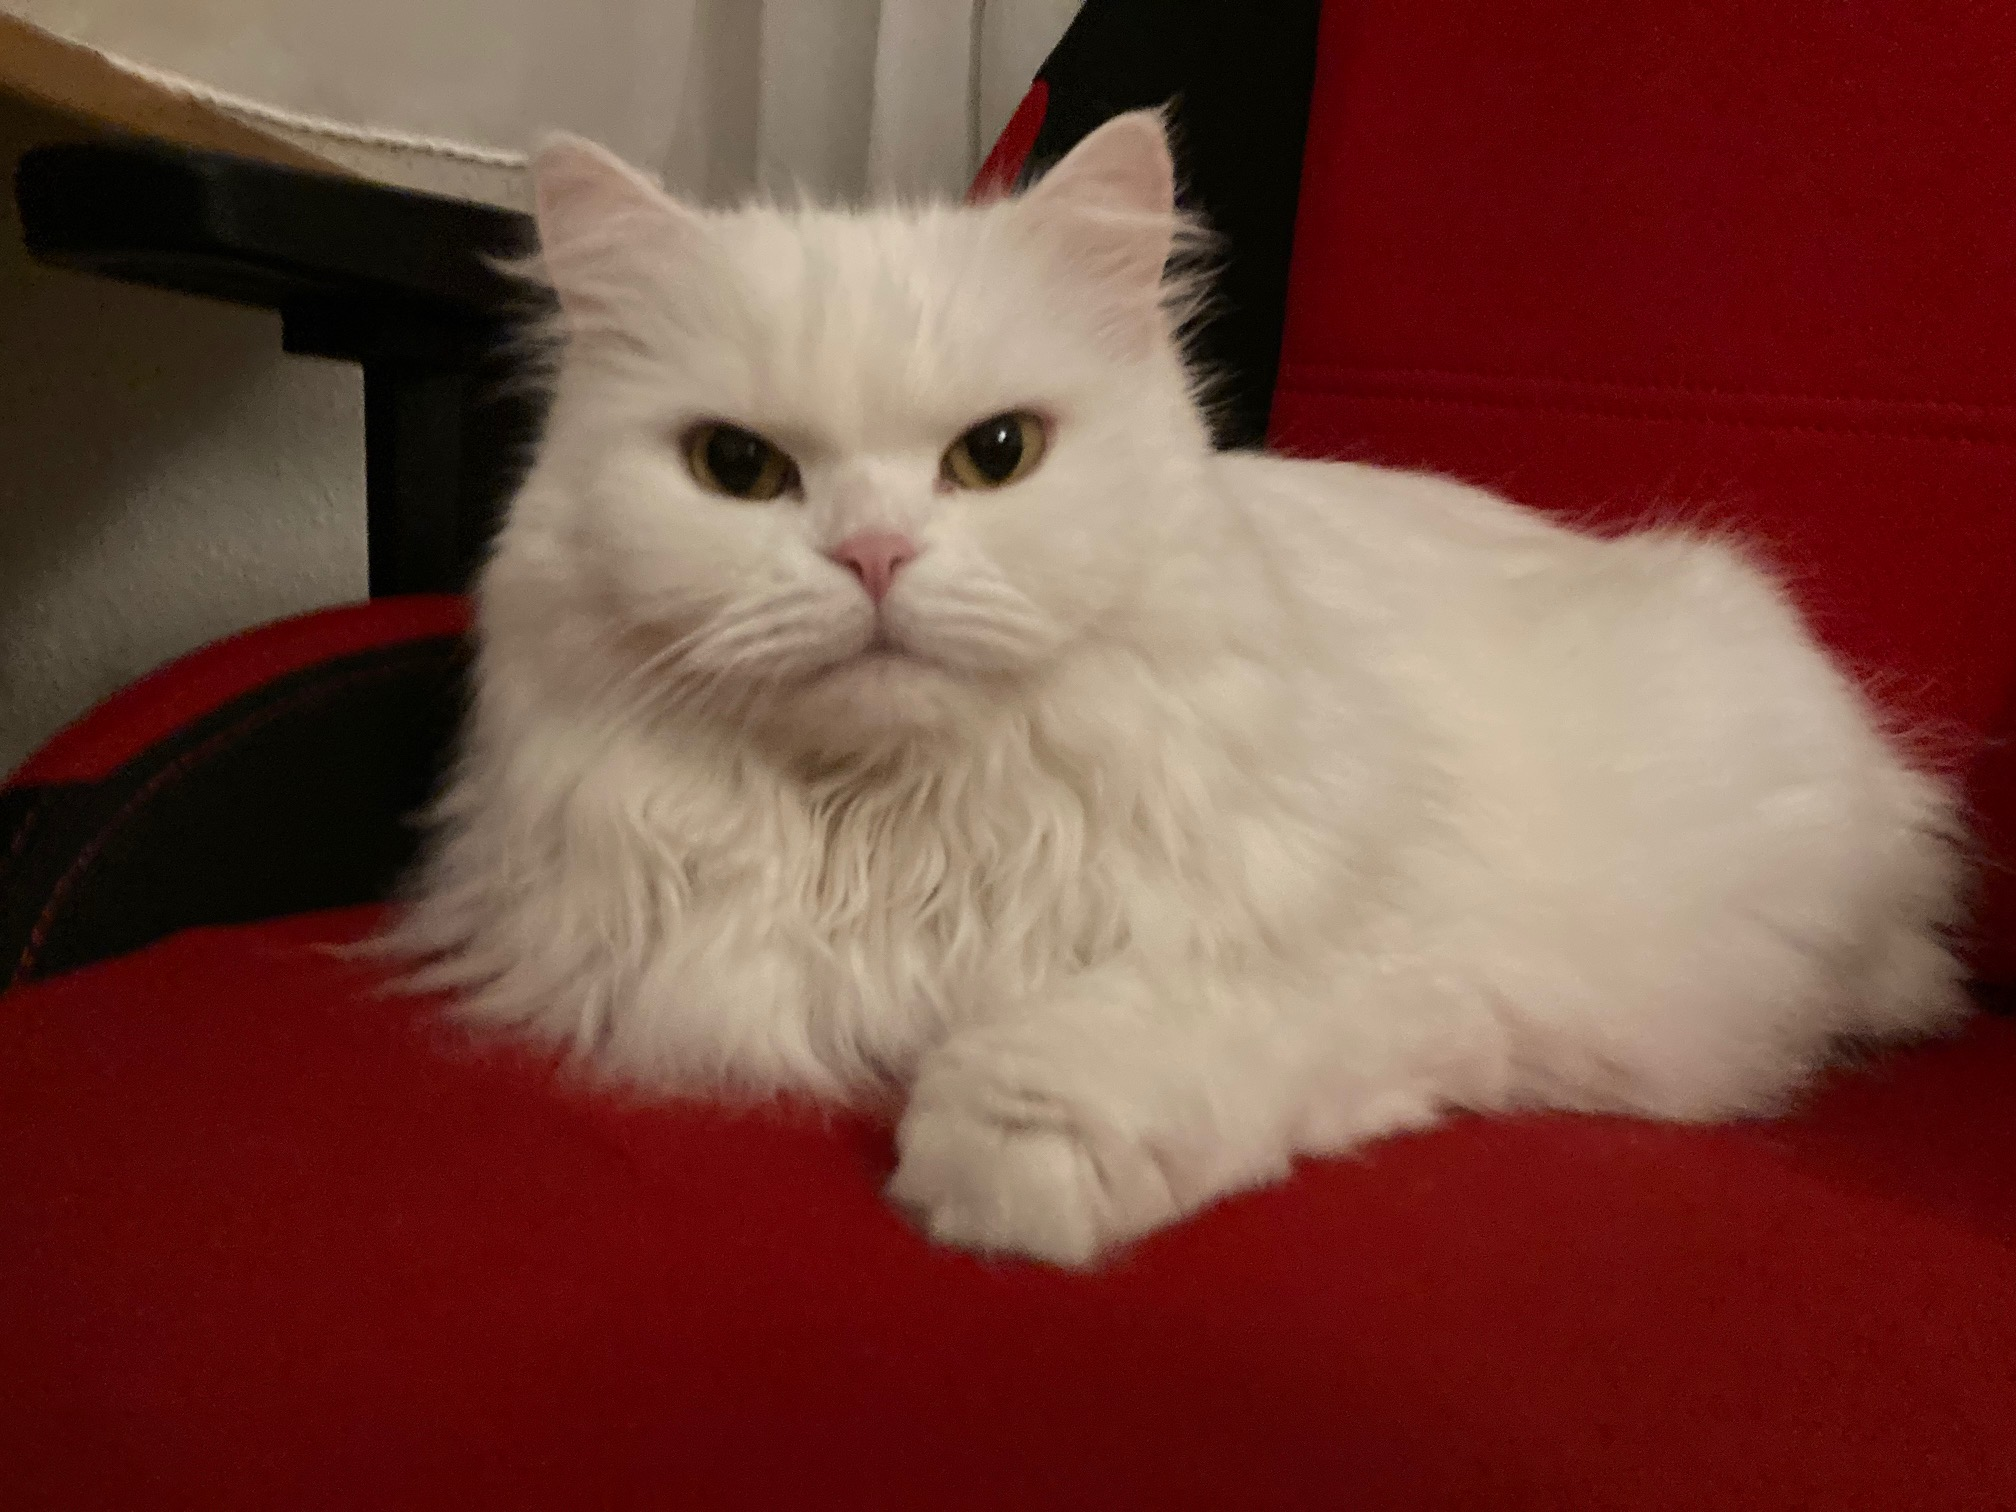
\includegraphics[width=\textwidth]{Bilder/Katze2}
\end{figure}

\blindtext[20]


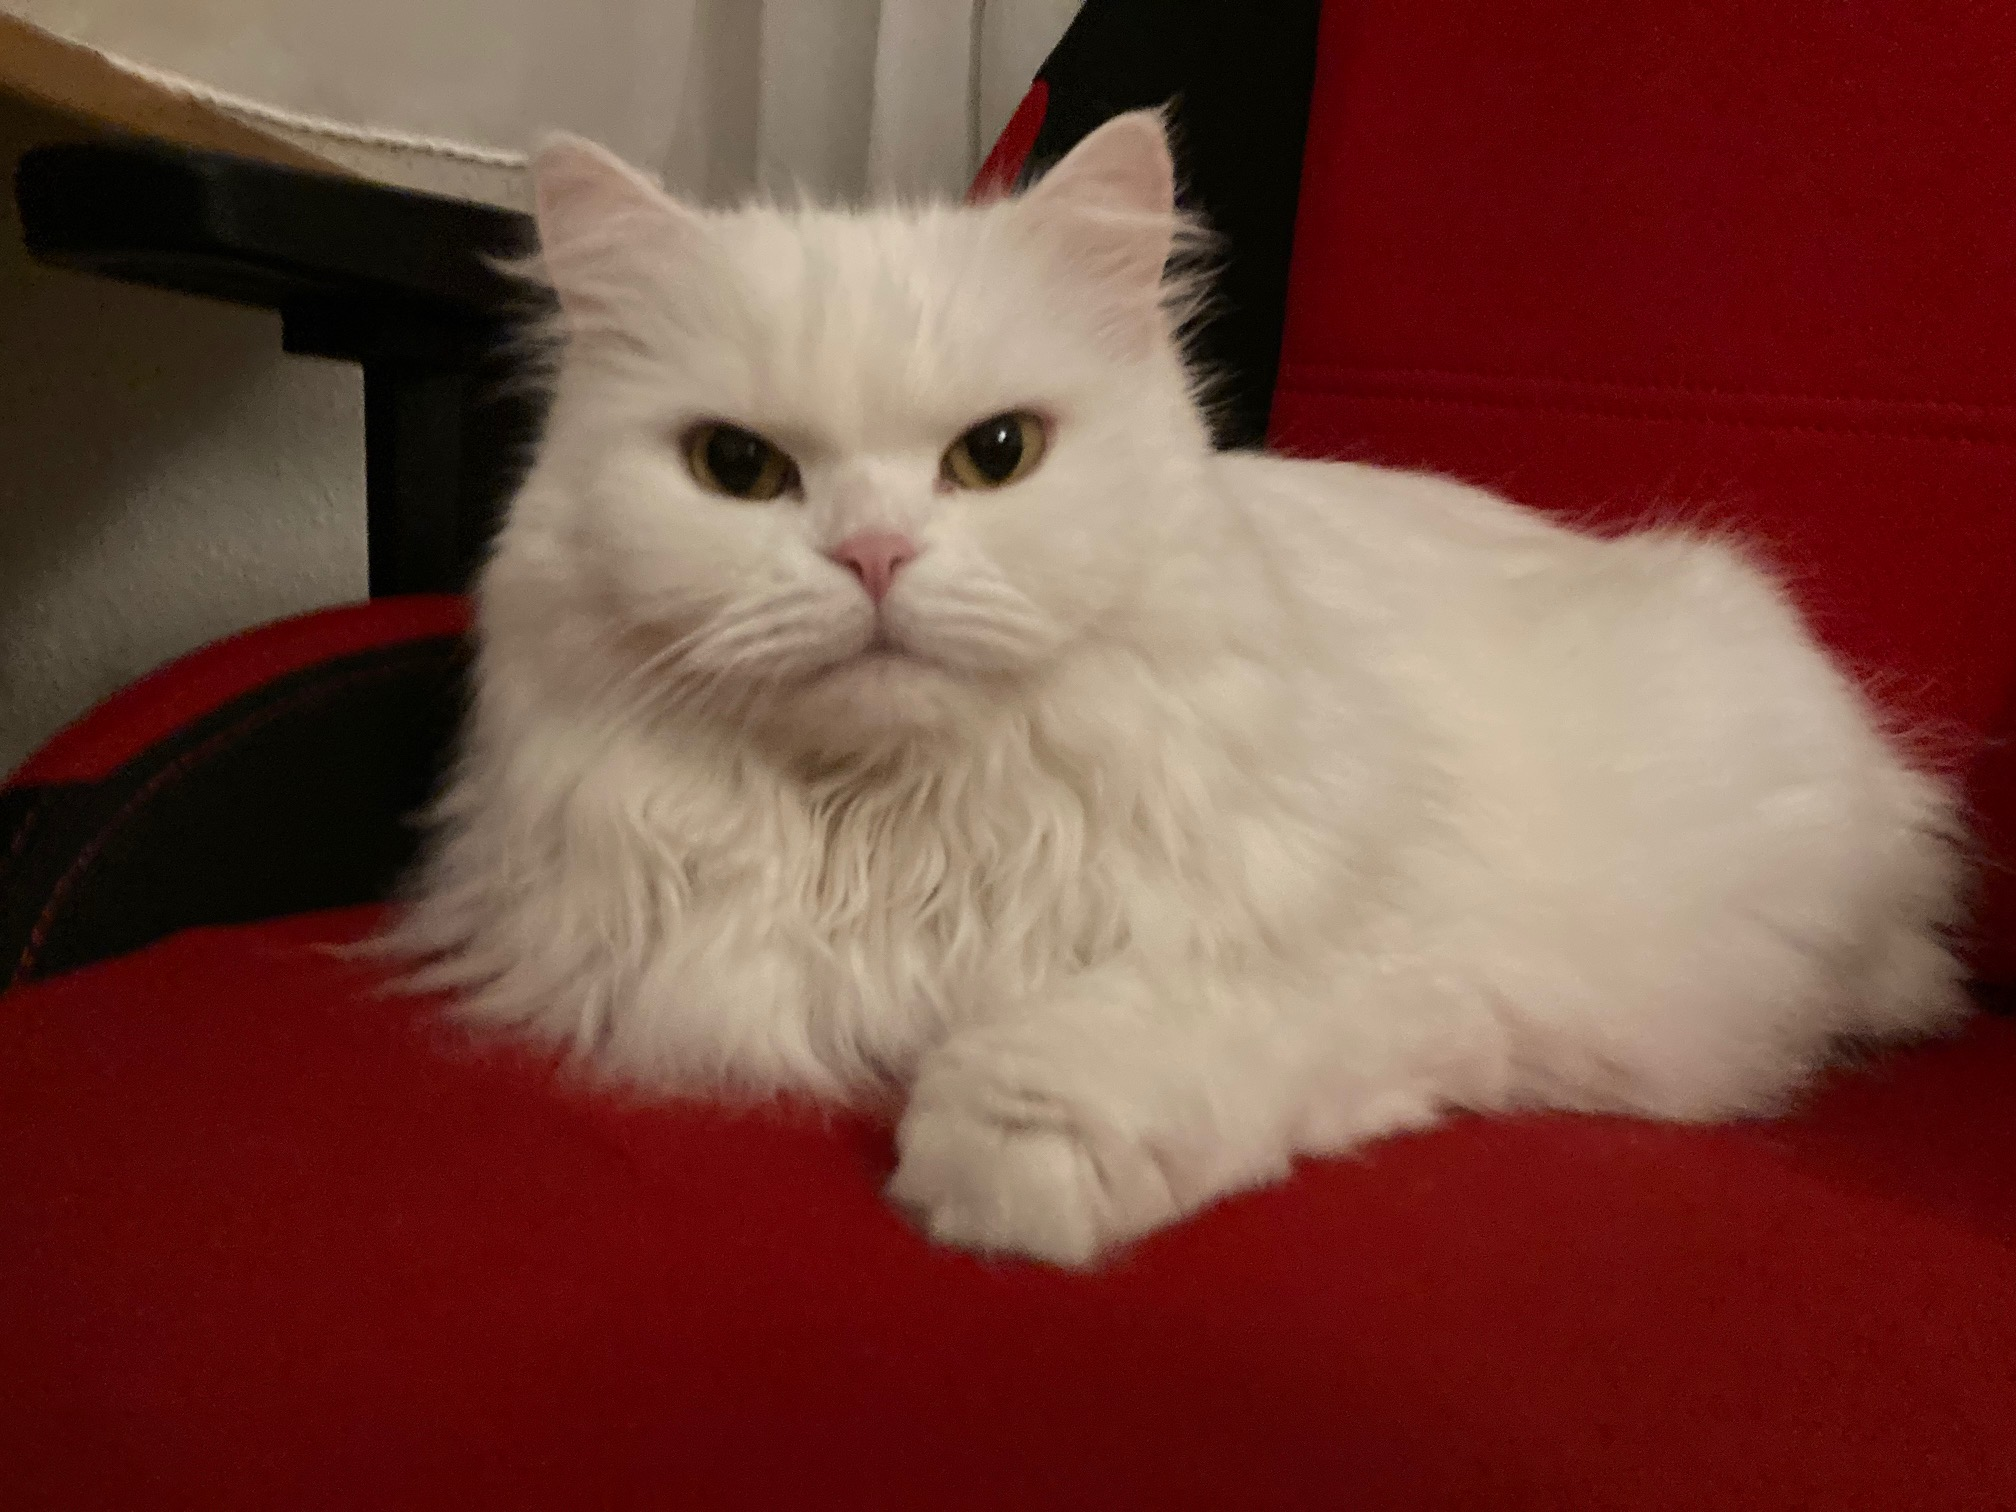
\includegraphics[width=\textwidth]{Bilder/Katze2}
\captionof{figure}{Meine Miezekatze}\label{fig:mieze}

\chapter{Mathematik}

TeX-Notation im Fließtest $a^2+b^2=c^2$ dsfisdh 

LaTeX-Notation im Fließtest \(a^2+b^2=c^2\) dsfisdh 

$$a^2+b^2=c^2$$

\[a^2+b^2=c^2\]

\[
\bordermatrix{%
    & 0 & 1 & 2 \cr
0 & A & B & C \cr
1 & A & B & C \cr
2 & A & B & C \cr
}
\]

\section{AMS Beispiele }

\[
\begin{pmatrix} 
A & B & C \\ 
A & B & C\\ 
A & B & C \\ 
\end{pmatrix}
\]

\[
\begin{bmatrix} 
A & B & C \\ 
A & B & C\\ 
A & B & C \\ 
\end{bmatrix}
\]

\[
\begin{Bmatrix} 
A & B & C \\ 
A & B & C\\ 
A & B & C \\ 
\end{Bmatrix}
\]

\begin{equation}\label{eq:sinnlos}
 z = \infty =  \det 
\begin{vmatrix} 
1 & 0 & 0 \\ 
0 & 1 & 0 \\ 
0 & 0 & 1 \\ 
\end{vmatrix}
\end{equation}

\[ \sum_{i=1}^{\infty^2} i ^3  \]

\[ z = \alpha \beta \gamma \pi 
\begin{Vmatrix} 
1 & 0 & 0 \\ 
0 & 1 & 0 \\ 
0 & 0 & 1 \\ 
\end{Vmatrix}
\]

% esvect Paket für den \vv{} Befehl

\[ \vec{a} \vv{a}  \cdot \vec{abc} \cdot \vv{abc} \]

\[  a \cap b  \cup c \rightarrow {x | x \text{ ist positiv}} \]

\[ A \not= \overline{A} \]

\[ ABC \not= \overline{ABC}  \Omega \]


Abstände im Mathematiksatz

\[ a b c \rightarrow abc \]

\[ a b c \Rightarrow a\,b\,c \]

\[ a b c \rightarrow a\;b\;c \]


\[ a b c \rightarrow a\quad b\quad c \]

\[ a b c \rightarrow a\qquad b\qquad c \]



\end{document}

